\documentclass[]{mattcv}

\usepackage{xcolor}
% flat ui colors
\definecolor{alizarin}{RGB}{231,76,60}
\definecolor{belizehole}{RGB}{41,128,185}
\definecolor{carrot}{RGB}{230,126,34}
\definecolor{emerald}{RGB}{46,204,113}
\definecolor{nephritis}{RGB}{39,174,96}
\definecolor{peterriver}{RGB}{52,152,220}
\definecolor{turquoise}{RGB}{26,188,156}
\definecolor{wetasphalt}{RGB}{52,73,94}

\usepackage{bbding}
\usepackage{dirtytalk}
\usepackage{everypage}
\usepackage[colorlinks=true, urlcolor=wetasphalt]{hyperref}
\usepackage[alpine, misc]{ifsym}
\usepackage{pgf-pie}
\usepackage{tikz}

\AddEverypageHook{%
    \cvheader
        {Mateusz} % first name(s)
        {Jemielity} % last name
        {40} % names fontsize
        {Software Engineer} % job title
        {20.3} % job title fontsize
        {matt.eps} % eps picture filepath
    }

\begin{document}

    \cvsection{contact}{wetasphalt}{%
        \begin{center}
            \FilledHut\hspace{2mm}Warszawa, Polska\hspace{1cm}\PhoneHandset\hspace{2mm}+01234567890\hspace{1cm}\Letter\hspace{2mm}email@example.com\\
            \href{https://google.com/+MateuszJemielity/about}{Google+: google.com/+MateuszJemielity}\hspace{1cm}\href{https://github.com/Matthew-Jemielity}{Github: github.com/Matthew-Jemielity}
        \end{center}
    }
    \cvsection{about}{carrot}{%
        \say{When you solve a puzzle the world makes sense and everything feels right.} (House MD)
        \par
        I'm an enthusiastic programmer and C is my language of choice, though I don't shy away from different ones. During my career I went from debugging to writing drivers, from making Linux kernel boot on new devices, to contributing to ambitious userland projects. I'm looking for an opportunity to expand my knowledge of the field and a chance to polish my skills.
    }
    \cvsection{experience}{emerald}{%
        \cvtimeline{\textbf{Senior Software Developer}, IS-Wireless}{nephritis}{2015}{now}{%
            \begin{itemize}
                \item responsible for architecture and implementation of 5G telecommunications software stack
                \item customized open source eNB and UE implementations
            \end{itemize}
        }
        \cvtimeline{\textbf{Software Engineer}, Samsung Electronics Poland R\&D Center}{nephritis}{2013}{2015}{%
            \begin{itemize}
                \item developed Linux kernel drivers and userland applications for GNU/Linux
                \item contributed to projects ranging from performance benchmarking to structured light 3D scanning
                \item investigated performance- and power consumption-related issues in ARM-based embedded systems
            \end{itemize}
        }
        \cvtimeline{\textbf{Junior Software Engineer}, Samsung Electronics Poland R\&D Center}{nephritis}{2009}{2013}{%
            \begin{itemize}
                \item implemented new features across proprietary bootloaders, L4-based RTOS, Android OS
                \item handled bringup of Linux kernel on new ARM-based hardware
                \item responsible for debugging and porting exisitng projects to new devices
            \end{itemize}
        }
    }
    \cvsection{education}{peterriver}{%
        \cvtimeline{\textbf{Informatics}, University of Gdańsk}{belizehole}{2004}{2009}{%
          \begin{itemize}
                \item uniform magister-level courses (MSc)
                \item \href{http://arch.ug.edu.pl/pl/najlepsi/index.php?strona=student&id_stud=526&lang=en}{best student 2008/2009}
                \item thesis title: \say{Turing Machine in Conway's Game of Life}
            \end{itemize}
        }
    }
    \cvsection{skills}{alizarin}{%
        \begin{center}
            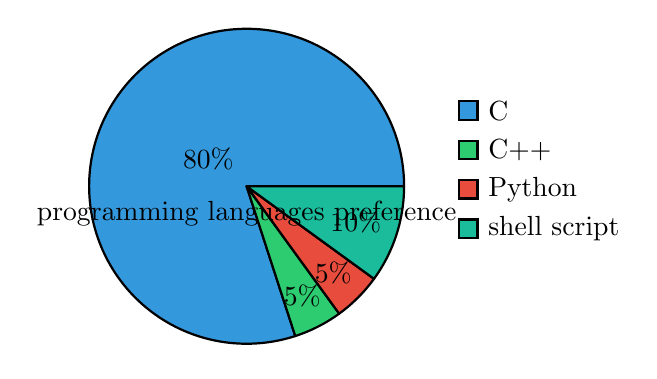
\begin{tikzpicture}
                \pie[
                    color={peterriver, emerald, alizarin, turquoise, carrot},
                    radius=2,
                    text=legend
                ]{80/C, 5/C++, 5/Python, 10/shell script}
                \node [below=2, align=flush center] {programming languages preference};
            \end{tikzpicture}
            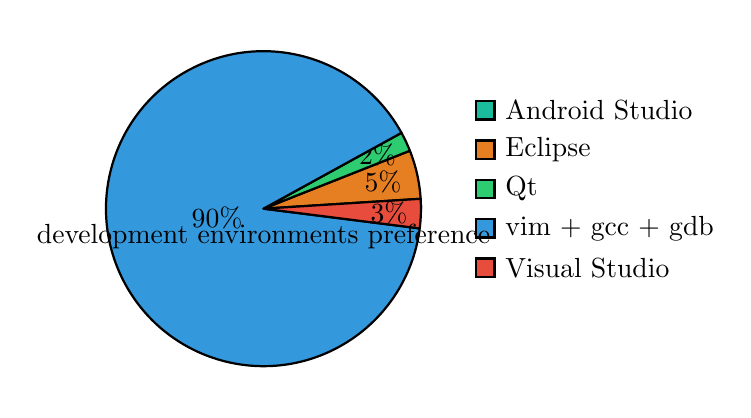
\begin{tikzpicture}
                \pie[
                    color={turquoise, carrot, emerald, peterriver, alizarin},
                    radius=2,
                    text=legend
                ]{1/Android Studio, 5/Eclipse, 2/Qt, 90/vim + gcc + gdb, 3/Visual Studio}
                \node [below=2, align=flush center] {development environments preference};
            \end{tikzpicture}
        \end{center}
    }

\end{document}

